\documentclass[aspectratio=169,10pt]{beamer}
% ----------------------------------------------------------------------
% Clean beamer theme + shared TikZ vocabulary for the Kimi Linear deck.
% ----------------------------------------------------------------------
\usetheme{default}
\usecolortheme{default}
\setbeamertemplate{navigation symbols}{}

\usepackage{lmodern}
\renewcommand{\familydefault}{\sfdefault}
\usepackage[T1]{fontenc}
\usepackage{amsmath,amssymb,bm}
\usepackage{booktabs}
\usepackage{tikz}
\usepackage{graphicx}
\usepackage{adjustbox}
\usetikzlibrary{arrows.meta,positioning,calc,fit,backgrounds,decorations.pathreplacing}

% A 16:9 beamer frame has only ~7cm of body height. Every diagram goes through
% \fig, which hard-caps its height (and width) so frames cannot overflow.
\newcommand{\fig}[2][3cm]{%
  \begin{center}%
  \adjustbox{max width=\linewidth,max totalheight=#1}{#2}%
  \end{center}%
}

% ---------------------------- palette ---------------------------------
\definecolor{ink}{RGB}{38,50,56}
\definecolor{accent}{RGB}{214,93,14}     % section accent (metropolis-ish)
\definecolor{gatered}{RGB}{178,34,34}    % the paper's "brickred" = gating
\definecolor{seagreen}{RGB}{20,110,114}
\definecolor{panel}{RGB}{245,246,247}
\definecolor{edge}{RGB}{198,204,208}
\definecolor{mute}{RGB}{120,132,138}

\setbeamercolor{normal text}{fg=ink}
\setbeamercolor{frametitle}{fg=ink}
\setbeamercolor{structure}{fg=accent}
\setbeamercolor{itemize item}{fg=accent}
\setbeamercolor{itemize subitem}{fg=mute}
\setbeamerfont{frametitle}{size=\large}
\setbeamerfont{title}{size=\LARGE}

% thin accent rule under every frame title
\setbeamertemplate{frametitle}{%
  \nointerlineskip\vspace{1.5em}%
  \hspace{0.9em}%
  \begin{minipage}{0.93\paperwidth}
    \usebeamerfont{frametitle}\usebeamercolor[fg]{frametitle}\insertframetitle\par
  \end{minipage}%
  \vspace{0.6em}%
}

\setbeamertemplate{footline}{%
  \makebox[\paperwidth][r]{%
    {\color{mute}\scriptsize\insertframenumber}\hspace*{1.2em}}%
  \vspace*{0.5em}%
}

\setbeamertemplate{itemize item}{\raisebox{0.12em}{\tiny$\blacksquare$}}
\setbeamertemplate{itemize subitem}{\raisebox{0.12em}{\tiny$\square$}}

% ---------------------------- macros ----------------------------------
\newcommand{\g}[1]{{\color{gatered}#1}}            % gating / decay terms
\newcommand{\hi}[1]{{\color{accent}#1}}            % what is new on this slide
\newcommand{\R}{\mathbb{R}}
\newcommand{\St}{\mathbf{S}}
\newcommand{\Diag}{\operatorname{Diag}}
\newcommand{\sm}{\operatorname{softmax}}
\newcommand{\Lo}{\mathcal{L}}

% a boxed side-note pinned to the bottom-right corner of a frame
\newcommand{\cornernote}[1]{%
  \begin{tikzpicture}[remember picture,overlay]
    \node[anchor=south east,xshift=-1.1em,yshift=1.6em,draw=edge,fill=panel,
          rounded corners=2pt,inner sep=5pt,font=\footnotesize,align=left]
      at (current page.south east) {#1};
  \end{tikzpicture}%
}

% a one-line takeaway banner
\newcommand{\takeaway}[1]{%
  \begin{center}
  \begin{tikzpicture}
    \node[draw=accent,fill=accent!6,rounded corners=3pt,inner sep=5pt,
          text width=0.86\paperwidth,align=center] {#1};
  \end{tikzpicture}
  \end{center}%
}

% inline numbered badge, matching the agenda callouts
\newcommand{\nb}[1]{\tikz[baseline=(n.base)]{\node[badge,inner sep=1pt,minimum size=3.8mm](n){#1};}}

% full-bleed section divider: orange canvas, white title
\newcommand{\sectionslide}[2]{%
  \begingroup
  \setbeamercolor{background canvas}{bg=accent}
  \setbeamertemplate{footline}{}
  \begin{frame}[plain]
    \vspace*{\fill}
    \begin{center}
      {\color{white!70!accent}\normalsize #1}\\[0.7em]
      {\color{white}\LARGE #2}
    \end{center}
    \vspace*{\fill}
  \end{frame}
  \endgroup
}

% ---------------------------- tikz styles ------------------------------
\tikzset{
  % VALUES (inputs / states / outputs): white fill
  val/.style   = {draw=edge,fill=white,rounded corners=2pt,inner sep=4pt,align=center},
  mat/.style   = {draw=edge,fill=white},
  % PARAMETERS (learned weight matrices): shaded fill
  wt/.style    = {draw=edge,fill=panel,rounded corners=2pt,inner sep=4pt,font=\small,align=center},
  % operations
  blk/.style   = {draw=edge,fill=panel,rounded corners=3pt,inner sep=6pt,align=center},
  % data-dependent gates are values, not parameters -> white fill, red border
  gate/.style  = {draw=gatered,fill=white,rounded corners=3pt,inner sep=5pt,
                  font=\small,text=gatered,align=center},
  arr/.style   = {-{Stealth[length=4pt]},draw=mute,thick},
  % MLA vs MHA: accent = low-rank compression path (new), red = decoupled RoPE
  newwt/.style = {wt,draw=accent,fill=accent!12,text=accent},
  lat/.style   = {val,draw=accent,text=accent,font=\small},
  rwt/.style   = {wt,draw=gatered,fill=gatered!12,text=gatered},
  rval/.style  = {val,draw=gatered,text=gatered,font=\small},
  arrnew/.style= {arr,draw=accent},
  arrrope/.style={arr,draw=gatered},
  badge/.style = {circle,fill=accent,text=white,inner sep=0pt,minimum size=4.6mm,
                  font=\footnotesize\bfseries},
  dim/.style   = {font=\footnotesize,text=mute},
  lbl/.style   = {font=\footnotesize},
}


\title{Kimi Linear}
\date{}
\author{}

\begin{document}

% ======================================================================
\begin{frame}[plain]
  \vspace{1.4cm}
  {\LARGE Kimi Linear}\\[0.35em]
  {\large\color{mute} An Expressive, Efficient Attention Architecture}\\[0.7em]
  {\color{accent}\rule{0.55\linewidth}{1.1pt}}\\[0.9em]
  {\footnotesize\color{mute} Kimi Team, November 2025 \quad$\cdot$\quad arXiv:2510.26692}\\[0.5em]
  {\footnotesize\color{mute} Presenter: Zhihan Yang}
\end{frame}

% ======================================================================
\begin{frame}[t]{Agenda}
\vspace{-0.1cm}
\begin{center}
\begin{tikzpicture}
  \node[anchor=south west,inner sep=0] (img) at (0,0)
        {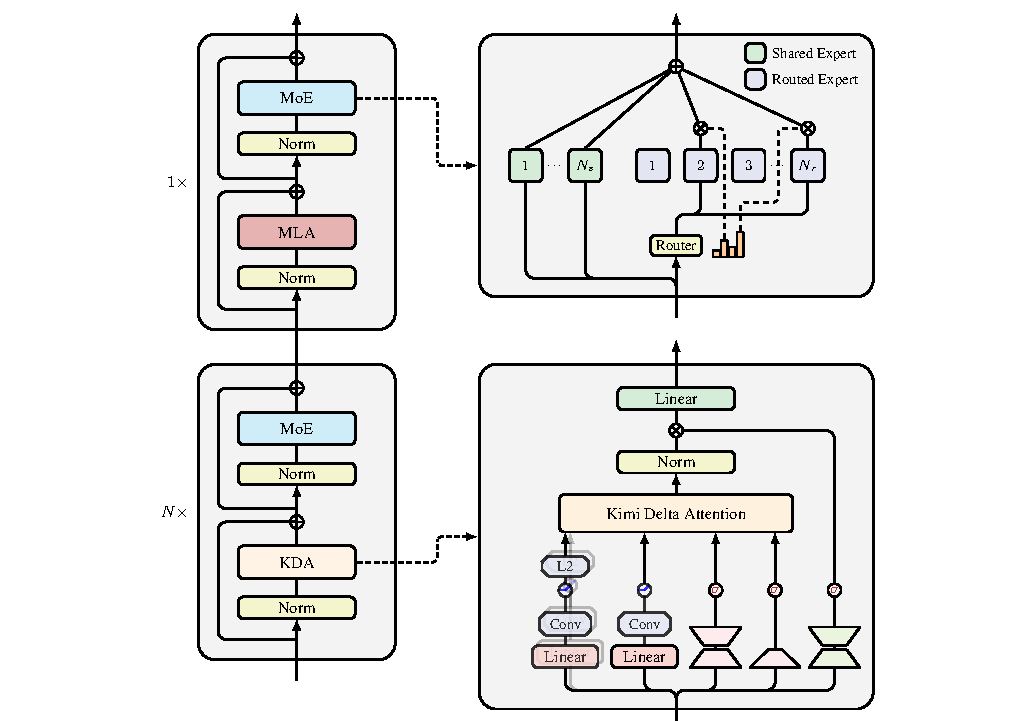
\includegraphics[height=0.605\paperheight]{fig-kimi-arch}};
  \begin{scope}[x={(img.south east)},y={(img.north west)}]
    \node[badge] at (0.105,0.865) {3};
    \node[badge] at (0.105,0.679) {1};
    \node[badge] at (0.105,0.407) {3};
    \node[badge] at (0.105,0.221) {2};
  \end{scope}
\end{tikzpicture}
\end{center}
\vspace{0.1cm}
{\scriptsize\centering
\nb{1}~Making Attention Cheaper (Still Quadratic)\hspace{1.1em}
\nb{2}~Making Linear Attention Work\hspace{1.1em}
\nb{3}~Making the MLP Cheaper\par}
\vspace{0.1cm}
{\scriptsize\color{mute}\centering Kimi Linear, Figure 3 --- 3 KDA layers per MLA layer, each followed by MoE.\par}
\end{frame}

\sectionslide{Section 1}{Making Attention Cheaper (Still Quadratic)}

% ======================================================================
\begin{frame}[t]{Multi-head self-attention (MHA)}
\vspace{0.15cm}
\begin{columns}[T]
\begin{column}{0.54\textwidth}
{\small
\[
  \bm{o}_t = \mathbf{W}_o\operatorname{Concat}_{h=1}^{H}\!\big(\bm{o}^h_t\big)\in\R^{d}
\]
\vspace{-0.45cm}
\[
  \bm{o}^h_t=\sum_{j\le t}\sm_{j\le t}\!\left(\frac{(\bm{q}^h_t)^\top \bm{k}^h_j}{\sqrt{d_k}}\right)\bm{v}^h_j\in\R^{d_v}
\]}
\vspace{-0.1cm}
\fig[3.0cm]{%
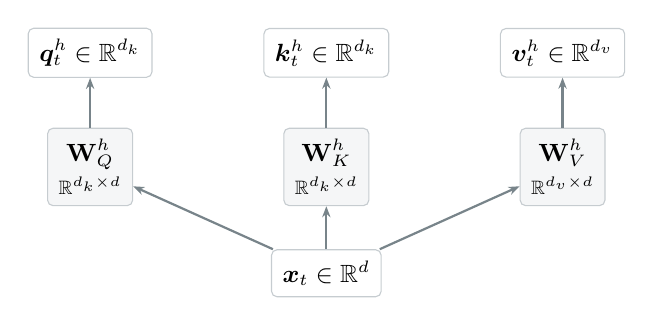
\begin{tikzpicture}[font=\small]
  \node[val] (x) at (0,0) {$\bm{x}_t\in\R^{d}$};
  \node[wt] (wq) at (-3.0,1.35) {$\mathbf{W}^h_Q$\\[1pt]{\scriptsize$\R^{d_k\times d}$}};
  \node[wt] (wk) at ( 0.0,1.35) {$\mathbf{W}^h_K$\\[1pt]{\scriptsize$\R^{d_k\times d}$}};
  \node[wt] (wv) at ( 3.0,1.35) {$\mathbf{W}^h_V$\\[1pt]{\scriptsize$\R^{d_v\times d}$}};
  \node[val] (q) at (-3.0,2.8) {$\bm{q}^h_t\in\R^{d_k}$};
  \node[val] (k) at ( 0.0,2.8) {$\bm{k}^h_t\in\R^{d_k}$};
  \node[val] (v) at ( 3.0,2.8) {$\bm{v}^h_t\in\R^{d_v}$};
  \foreach \a/\b in {x/wq,x/wk,x/wv,wq/q,wk/k,wv/v} \draw[arr] (\a) -- (\b);
\end{tikzpicture}}
\end{column}

\begin{column}{0.46\textwidth}
\vspace{0.2cm}
\fig[3.0cm]{%
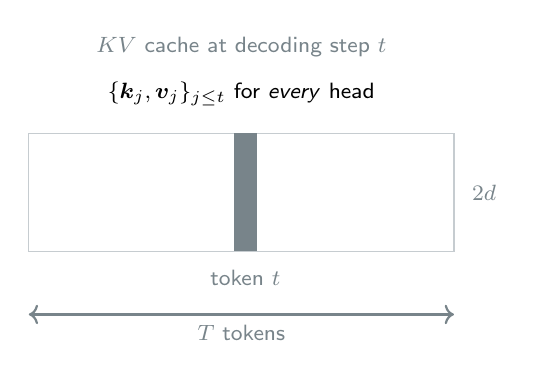
\begin{tikzpicture}
  \node[font=\footnotesize,text=mute] at (2.7,2.6) {$KV$ cache at decoding step $t$};
  \node[font=\footnotesize] at (2.7,2.0) {$\{\bm{k}_j,\bm{v}_j\}_{j\le t}$ for \emph{every} head};
  \draw[mat] (0,0) rectangle (5.4,1.5);
  \fill[mute] (2.6,0) rectangle (2.9,1.5);
  \node[dim,right=3pt] at (5.4,0.75) {$2d$};
  \node[dim] at (2.75,-0.33) {token $t$};
  \draw[arr,<->] (0,-0.8) -- (5.4,-0.8) node[midway,below,dim] {$T$ tokens};
\end{tikzpicture}}
\vspace{0.3cm}
{\small
\begin{itemize}
  \item Cache cost grows \textbf{linearly in $T$}.
  \item Per-step compute grows linearly too.
  \item $d_k=d_v=d/H$.
\end{itemize}}
\end{column}
\end{columns}
\end{frame}

% ======================================================================
\begin{frame}[t]{Multi-head latent attention (MLA) --- Training}
\vspace{0.05cm}
\begin{columns}[T]
% ---------------------------------------------------------------- MHA
\begin{column}{0.39\textwidth}
{\footnotesize\centering\textbf{MHA}\par}
\fig[2.6cm]{%
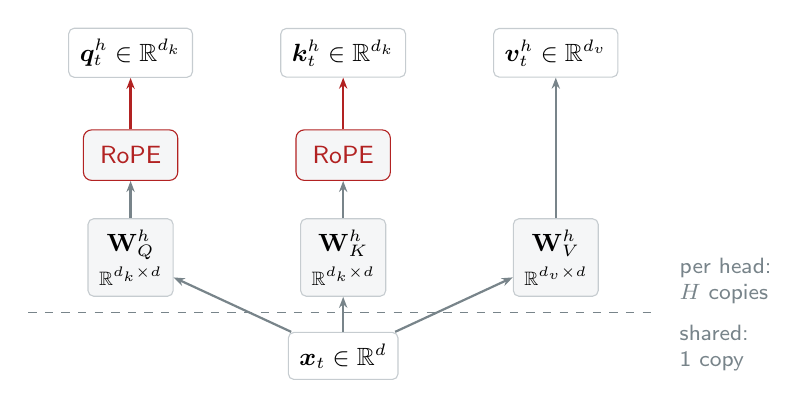
\begin{tikzpicture}[font=\small]
  \node[val] (x) at (0,0) {$\bm{x}_t\in\R^{d}$};
  \node[wt] (wq) at (-2.7,1.25) {$\mathbf{W}^h_Q$\\[1pt]{\scriptsize$\R^{d_k\times d}$}};
  \node[wt] (wk) at ( 0.0,1.25) {$\mathbf{W}^h_K$\\[1pt]{\scriptsize$\R^{d_k\times d}$}};
  \node[wt] (wv) at ( 2.7,1.25) {$\mathbf{W}^h_V$\\[1pt]{\scriptsize$\R^{d_v\times d}$}};
  % RoPE applies to the FULL q and k here
  \node[blk,draw=gatered,text=gatered,font=\small] (rq) at (-2.7,2.55) {RoPE};
  \node[blk,draw=gatered,text=gatered,font=\small] (rk) at ( 0.0,2.55) {RoPE};
  \node[val] (q) at (-2.7,3.85) {$\bm{q}^h_t\in\R^{d_k}$};
  \node[val] (k) at ( 0.0,3.85) {$\bm{k}^h_t\in\R^{d_k}$};
  \node[val] (v) at ( 2.7,3.85) {$\bm{v}^h_t\in\R^{d_v}$};
  \foreach \a/\b in {x/wq,x/wk,x/wv,wq/rq,wk/rk,wv/v} \draw[arr] (\a) -- (\b);
  \draw[arrrope] (rq) -- (q);  \draw[arrrope] (rk) -- (k);
  % head split happens immediately: only x_t sits below the line
  \draw[dashed,draw=mute] (-4.0,0.55) -- (4.0,0.55);
  \node[dim,anchor=west,align=left] at (4.15,0.95) {per head:\\ $H$ copies};
  \node[dim,anchor=west,align=left] at (4.15,0.1) {shared:\\ 1 copy};
\end{tikzpicture}}
\vspace{0.05cm}
{\scriptsize\color{mute}\centering RoPE rotates the \emph{whole} $\bm{q},\bm{k}$.\par}
\end{column}

% ---------------------------------------------------------------- MLA
\begin{column}{0.61\textwidth}
{\footnotesize\centering\textbf{MLA}\par}
\fig[3.7cm]{%
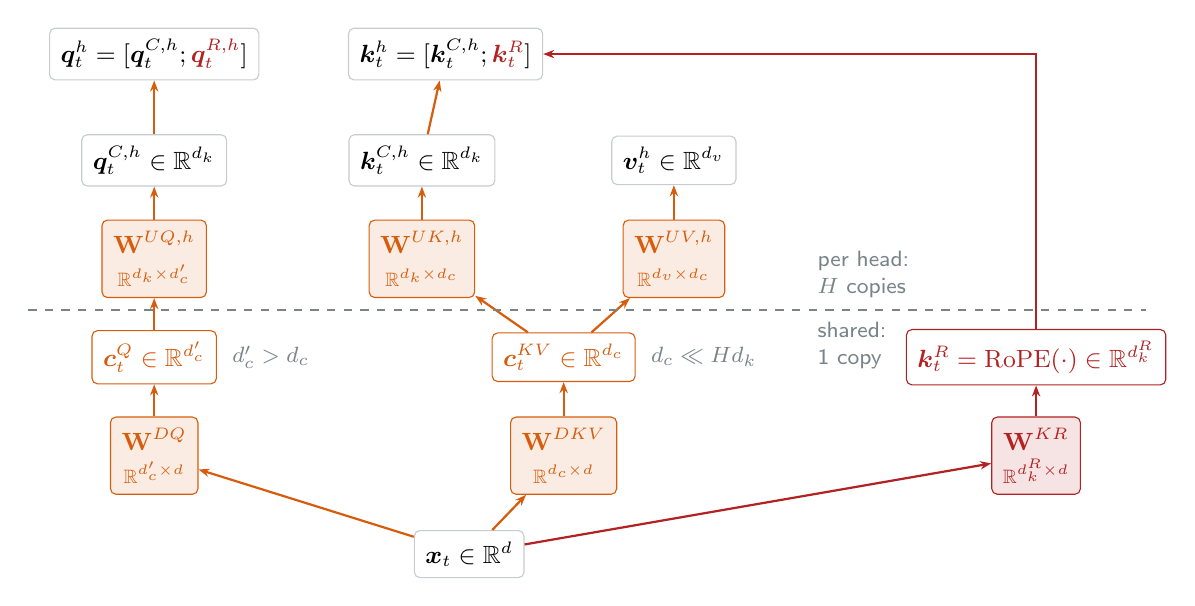
\begin{tikzpicture}[font=\small]
  \node[val] (x) at (0,0) {$\bm{x}_t\in\R^{d}$};
  \node[newwt] (wdq)  at (-4.0,1.25) {$\mathbf{W}^{DQ}$\\[1pt]{\scriptsize$\R^{d'_c\times d}$}};
  \node[newwt] (wdkv) at ( 1.2,1.25) {$\mathbf{W}^{DKV}$\\[1pt]{\scriptsize$\R^{d_c\times d}$}};
  \node[rwt]   (wkr)  at ( 7.2,1.25) {$\mathbf{W}^{KR}$\\[1pt]{\scriptsize$\R^{d^R_k\times d}$}};
  \node[lat]   (cq)   at (-4.0,2.5) {$\bm{c}^{Q}_t\in\R^{d'_c}$};
  \node[lat]   (ckv)  at ( 1.2,2.5) {$\bm{c}^{KV}_t\in\R^{d_c}$};
  \node[rval]  (kr)   at ( 7.2,2.5) {$\g{\bm{k}^R_t}=\mathrm{RoPE}(\cdot)\in\R^{d^R_k}$};
  \node[newwt] (wuq) at (-4.0,3.75) {$\mathbf{W}^{UQ,h}$\\[1pt]{\scriptsize$\R^{d_k\times d'_c}$}};
  \node[newwt] (wuk) at (-0.6,3.75) {$\mathbf{W}^{UK,h}$\\[1pt]{\scriptsize$\R^{d_k\times d_c}$}};
  \node[newwt] (wuv) at ( 2.6,3.75) {$\mathbf{W}^{UV,h}$\\[1pt]{\scriptsize$\R^{d_v\times d_c}$}};
  \node[val] (q) at (-4.0,5.0) {$\bm{q}^{C,h}_t\in\R^{d_k}$};
  \node[val] (k) at (-0.6,5.0) {$\bm{k}^{C,h}_t\in\R^{d_k}$};
  \node[val] (v) at ( 2.6,5.0) {$\bm{v}^{h}_t\in\R^{d_v}$};
  % concatenation of the content half with the RoPE half
  \node[val] (qcat) at (-4.0,6.35) {$\bm{q}^h_t=[\bm{q}^{C,h}_t;\g{\bm{q}^{R,h}_t}]$};
  \node[val] (kcat) at (-0.3,6.35) {$\bm{k}^h_t=[\bm{k}^{C,h}_t;\g{\bm{k}^R_t}]$};
  \foreach \a/\b in {x/wdq,x/wdkv,wdq/cq,wdkv/ckv,cq/wuq,ckv/wuk,ckv/wuv,
                     wuq/q,wuk/k,wuv/v} \draw[arrnew] (\a) -- (\b);
  \draw[arrrope] (x) -- (wkr);   \draw[arrrope] (wkr) -- (kr);
  \draw[arrnew] (q) -- (qcat);   \draw[arrnew] (k) -- (kcat);
  \draw[arrrope] (kr.north) |- (kcat.east);
  \node[dim,right=2pt of cq] {$d'_c>d_c$};
  \node[dim,right=2pt of ckv] {$d_c\ll Hd_k$};
  % the head dimension is created at the up-projection, not carried from below
  \draw[dashed,draw=mute] (-5.6,3.1) -- (8.6,3.1);
  \node[dim,anchor=west,align=left] at (4.3,3.55) {per head:\\ $H$ copies};
  \node[dim,anchor=west,align=left] at (4.3,2.65) {shared:\\ 1 copy};
\end{tikzpicture}}
\vspace{0.05cm}
{\scriptsize\centering
\textcolor{accent}{$\blacksquare$}~low-rank compression\quad
\textcolor{gatered}{$\blacksquare$}~decoupled RoPE\quad
{\color{mute}$D$: \textbf{d}own\ $\cdot$\ $U$: \textbf{u}p\ $\cdot$\ $R$: \textbf{R}oPE}\par
\vspace{1pt}
{\color{gatered}But now position enters \emph{only} through the $d^R_k$ dimensions
($\bm{q}^{R,h}_t$ is RoPE of $\bm{c}^Q_t$)\par}}
\end{column}
\end{columns}

\vspace{0.35cm}
{\centering
{\footnotesize\hi{Intuition:} MLA is MHA with every projection factorized through a low-rank latent ($\hi{\bm{c}^{Q}_t}$, $\hi{\bm{c}^{KV}_t}$)\par}
\vspace{3pt}
{\small$\mathbf{W}^{\hi{h}}_Q\approx\mathbf{W}^{UQ,\hi{h}}\mathbf{W}^{DQ}$
\quad
$\mathbf{W}^{\hi{h}}_K\approx\mathbf{W}^{UK,\hi{h}}\mathbf{W}^{DKV}$
\quad
$\mathbf{W}^{\hi{h}}_V\approx\mathbf{W}^{UV,\hi{h}}\mathbf{W}^{DKV}$\par}

}
\end{frame}

% ======================================================================
\begin{frame}[t]{MLA vs MHA: measured quality and cache}
\vspace{0.05cm}
\begin{center}
{\footnotesize
\begin{tabular}{@{}lcccc@{}}
\toprule
 & \multicolumn{2}{c}{Small MoE (1.33T tokens)} & \multicolumn{2}{c}{Large MoE (420B tokens)}\\
\cmidrule(lr){2-3}\cmidrule(lr){4-5}
 & MHA & \hi{MLA} & MHA & \hi{MLA}\\
\midrule
Activated params  & 2.5B   & \hi{2.4B}  & 25.0B  & \hi{21.5B}\\
KV cache / token  & 110.6K & \hi{15.6K} & 860.2K & \hi{34.6K}\\
\midrule
BBH     & 37.9 & \hi{39.0} & 46.6 & \hi{50.7}\\
MMLU    & 48.7 & \hi{50.0} & 57.5 & \hi{59.0}\\
C-Eval  & 51.6 & 50.9      & 57.9 & \hi{59.2}\\
CMMLU   & 52.3 & \hi{53.4} & 60.7 & \hi{62.5}\\
\bottomrule
\end{tabular}}
\end{center}
\vspace{0.1cm}
{\scriptsize\color{mute}\centering DeepSeek-V2, Appendix D (Tables 8--9). Attention swapped in place --- same depth, width, heads, data; params land where they land, so MLA is handicapped.\par}
\vspace{0.1cm}
{\footnotesize
\begin{itemize}
  \item MLA wins 7 of 8, with \emph{fewer} activated params; cache falls to \textbf{14\%} / \textbf{4\%} of MHA (independent of $T$).
  \item Margin widens with scale ($+0.7\to+2.4$) --- but two points is not a scaling law.
  \item 7B dense: MHA $>$ GQA $>$ MQA on MMLU ($45.2/41.2/37.9$) --- cheaper caches usually cost quality.
  \item \g{Caveat:} only these four (three multiple-choice, all short-context) --- where a compressed cache is \emph{not} stressed. GSM8K/MATH/HumanEval appear only for the shipped model, no MHA baseline.
\end{itemize}}
\end{frame}

% ======================================================================
\begin{frame}[t]{Multi-head latent attention (MLA) --- Inference}
\vspace{0.1cm}
{\small Past tokens are \hi{never expanded back} into $\bm{k},\bm{v}$ --- attention runs on the latent.}

\begin{columns}[T]
\begin{column}{0.52\textwidth}
\vspace{0.05cm}
{\footnotesize\textbf{Scores: the two halves are handled differently.}}
{\scriptsize
\[
  \bm{q}^{h\top}_t\bm{k}^h_j\;=\;
  \big(\underbrace{\bm{q}^{C,h\top}_t\mathbf{W}^{UK,h}}_{\text{fold: once per step}}\big)\,\bm{c}^{KV}_j
  \;+\;\underbrace{\g{\bm{q}^{R,h\top}_t\,\bm{k}^R_j}}_{\text{vs.\ cached }\g{\bm{k}^R_j}}
\]}
\vspace{0.1cm}
{\footnotesize\textbf{Values: pull $\mathbf{W}^{UV}$ out of the sum.}}
{\footnotesize
\[
  \sum_{j\le t} a_j\big(\mathbf{W}^{UV,h}\bm{c}^{KV}_j\big)
  \;=\;\mathbf{W}^{UV,h}\Big(\sum_{j\le t} a_j\,\bm{c}^{KV}_j\Big)
\]}
\vspace{-0.2cm}
{\footnotesize
\begin{itemize}
  \item The fold depends on $t$, not $j$: done \textbf{once} per step.
  \item Only the \emph{content} half is absorbed; under \textbf{NoPE} the second term vanishes.
  \item $\bm{k}^{C,h}_j,\bm{v}^{h}_j$ are never stored \emph{and never rebuilt}.
  \item $\bm{c}^{Q}_t$ is \textbf{not} cached --- queries are current-token only.
\end{itemize}}
\end{column}

\begin{column}{0.48\textwidth}
\vspace{0.3cm}
\fig[3.1cm]{%
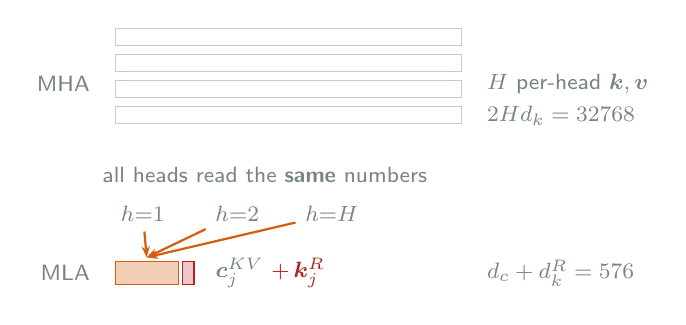
\begin{tikzpicture}[font=\footnotesize]
  % MHA: one cache per head
  \node[dim,anchor=east] at (-0.2,3.75) {MHA};
  \foreach \i in {0,1,2,3}
    \draw[mat] (0,{3.25+0.33*\i}) rectangle (4.4,{3.47+0.33*\i});
  \node[dim,anchor=west] at (4.6,3.75) {$H$ per-head $\bm{k},\bm{v}$};
  \node[dim,anchor=west] at (4.6,3.35) {$2Hd_k=32768$};

  % MLA: every head reads the same latent
  \foreach \x/\lab in {0.35/$h{=}1$,1.55/$h{=}2$,2.75/$h{=}H$}
    {\node[dim] (hd) at (\x,2.1) {\lab};
     \draw[arr,draw=accent] (hd) -- (0.4,1.55);}
  \node[dim] at (1.9,2.6) {all heads read the \textbf{same} numbers};
  \node[dim,anchor=east] at (-0.2,1.35) {MLA};
  \draw[mat,fill=accent!30,draw=accent] (0,1.2) rectangle (0.8,1.5);
  \draw[mat,fill=gatered!25,draw=gatered] (0.85,1.2) rectangle (1.0,1.5);
  \node[dim,anchor=west] at (4.6,1.35) {$d_c+d^R_k=576$};
  \node[dim,anchor=west] at (1.15,1.35) {$\bm{c}^{KV}_j$ \g{$+\,\bm{k}^R_j$}};
\end{tikzpicture}}
{\scriptsize\color{mute}\centering DeepSeek-V3 config; traffic per token, per layer\par}
\vspace{0.1cm}
{\footnotesize
\begin{itemize}
  \item This is exactly \textbf{MQA} with head dim $d_c$.
  \item Decoding is bandwidth-bound: $\sim$57$\times$ less traffic per step.
\end{itemize}}
\end{column}
\end{columns}

\end{frame}

\sectionslide{Section 2}{Making Linear Attention Work}

% ======================================================================
\begin{frame}[t]{Linear attention: a fixed-size state}
\vspace{0.1cm}
{\small Drop the softmax. Keep a \hi{matrix-valued state} $\St_t\in\R^{d_k\times d_v}$ instead of a growing cache.}

\begin{columns}[T]
\begin{column}{0.5\textwidth}
{\small
\[
  \St_t=\St_{t-1}+\bm{k}_t\bm{v}^\top_t,\qquad \bm{o}_t=\St^\top_t\bm{q}_t
\]}
\vspace{-0.15cm}
\fig[2.0cm]{%
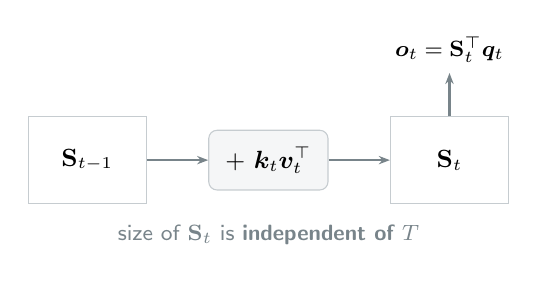
\begin{tikzpicture}[font=\small]
  \node[mat,minimum width=1.5cm,minimum height=1.1cm] (s0) at (0,0) {$\St_{t-1}$};
  \node[blk] (plus) at (2.3,0) {$+\ \bm{k}_t\bm{v}^\top_t$};
  \node[mat,minimum width=1.5cm,minimum height=1.1cm] (s1) at (4.6,0) {$\St_{t}$};
  \draw[arr] (s0) -- (plus); \draw[arr] (plus) -- (s1);
  \draw[arr] (s1.north) -- ++(0,0.55) node[above,font=\footnotesize] {$\bm{o}_t=\St^\top_t\bm{q}_t$};
  \node[dim] at (2.3,-0.95) {size of $\St_t$ is \textbf{independent of $T$}};
\end{tikzpicture}}
\vspace{0.15cm}
{\footnotesize
\begin{itemize}
  \item $\St_t$ is an \emph{associative memory}: key $\mapsto$ value.
  \item $O(1)$ memory, $O(1)$ compute per token.
\end{itemize}}
\end{column}

\begin{column}{0.5\textwidth}
{\small\textbf{Online-learning view.} The update is gradient \emph{descent} on
\[
  \Lo_t(\St)=-\langle \St^\top\bm{k}_t,\ \bm{v}_t\rangle
\]}
\vspace{-0.25cm}
\fig[1.2cm]{%
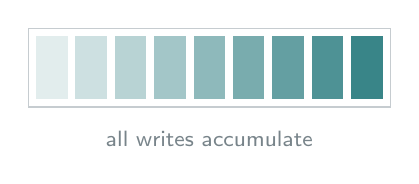
\begin{tikzpicture}[font=\footnotesize]
  \draw[mat] (0,0) rectangle (4.6,1.0);
  \foreach \i in {0,...,8}
    \fill[seagreen,draw=none,opacity={0.12+0.09*\i}]
      ({0.1+0.5*\i},0.1) rectangle ({0.5+0.5*\i},0.9);
  \node[dim] at (2.3,-0.4) {all writes accumulate};
\end{tikzpicture}}
\vspace{0.1cm}
{\footnotesize
\begin{itemize}
  \item No criterion for \emph{what to erase}.
  \item Associations interfere over long contexts.
\end{itemize}}
\end{column}
\end{columns}

\vfill
\takeaway{Fixed memory, but no forgetting and no error correction.}
\end{frame}

% ======================================================================
\begin{frame}[t]{DeltaNet: error-correcting updates}
\vspace{0.1cm}
{\small Replace the correlation objective with a \hi{reconstruction loss}:
$\ \Lo_t(\St)=\tfrac12\lVert \St^\top\bm{k}_t-\bm{v}_t\rVert^2$.}

\begin{columns}[T]
\begin{column}{0.54\textwidth}
\vspace{0.1cm}
{\small One gradient step with learning rate $\beta_t$:
\[
  \St_t=\St_{t-1}-\beta_t\nabla_{\St}\Lo_t(\St_{t-1})
      =\big(\mathbf{I}-\hi{\beta_t\bm{k}_t\bm{k}^\top_t}\big)\St_{t-1}+\beta_t\bm{k}_t\bm{v}^\top_t
\]
Equivalently, as an \emph{error-correcting} write:
\[
  \St_t=\St_{t-1}+\beta_t\,\bm{k}_t\big(\underbrace{\bm{v}_t-\St^\top_{t-1}\bm{k}_t}_{\text{prediction error}}\big)^{\!\top}
\]}
\vspace{0.05cm}
{\small
\begin{itemize}
  \item $\mathbf{I}-\beta_t\bm{k}_t\bm{k}^\top_t$ is a generalized \textbf{Householder} transform: erase along $\bm{k}_t$ only.
  \item Rank-1 structure $\Rightarrow$ chunkwise parallel training.
\end{itemize}}
\end{column}

\begin{column}{0.46\textwidth}
\vspace{0.3cm}
\fig[3.3cm]{%
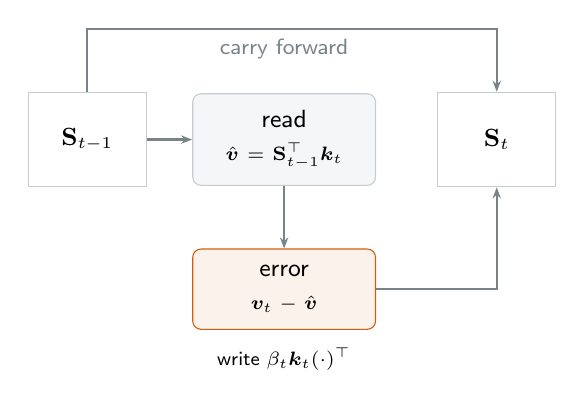
\begin{tikzpicture}[font=\small]
  \node[mat,minimum width=1.5cm,minimum height=1.2cm] (s0) at (0,0) {$\St_{t-1}$};
  \node[blk,text width=1.9cm] (rd) at (2.5,0) {read\\[1pt]{\scriptsize $\hat{\bm{v}}=\St^\top_{t-1}\bm{k}_t$}};
  \node[blk,text width=1.9cm,draw=accent,fill=accent!8] (er) at (2.5,-1.9)
       {error\\[1pt]{\scriptsize $\bm{v}_t-\hat{\bm{v}}$}};
  \node[mat,minimum width=1.5cm,minimum height=1.2cm] (s1) at (5.2,0) {$\St_{t}$};
  \draw[arr] (s0) -- (rd);
  \draw[arr] (rd) -- (er);
  \draw[arr] (er.east) -| (s1.south);
  \node[font=\scriptsize,below=3pt of er] {write $\beta_t\bm{k}_t(\cdot)^\top$};
  \draw[arr] (s0.north) -- ++(0,0.8) -| (s1.north);
  \node[dim] at (2.5,1.15) {carry forward};
\end{tikzpicture}}
\vspace{0.1cm}
{\footnotesize\color{mute}\centering If $\St_{t-1}$ already predicts $\bm{v}_t$, nothing is written.\par}
\end{column}
\end{columns}

\vfill
\takeaway{Error correction, but old associations persist indefinitely.}
\end{frame}

% ======================================================================
\begin{frame}[t]{Gated DeltaNet: scalar decay}
\vspace{0.1cm}
{\small Add a data-dependent forget gate \g{$\alpha_t\in[0,1]$} --- a \hi{scalar} per token.}

\begin{columns}[T]
\begin{column}{0.54\textwidth}
\vspace{0.15cm}
{\small
\[
  \St_t=\g{\alpha_t}\big(\mathbf{I}-\beta_t\bm{k}_t\bm{k}^\top_t\big)\St_{t-1}+\beta_t\bm{k}_t\bm{v}^\top_t
\]}
\vspace{-0.15cm}
\fig[2.0cm]{%
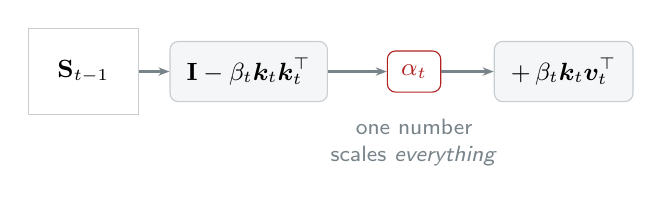
\begin{tikzpicture}[font=\small]
  \node[mat,minimum width=1.4cm,minimum height=1.1cm] (s0) at (0,0) {$\St_{t-1}$};
  \node[blk] (h) at (2.1,0) {$\mathbf{I}-\beta_t\bm{k}_t\bm{k}^\top_t$};
  \node[gate] (a) at (4.2,0) {\g{$\alpha_t$}};
  \node[blk] (w) at (6.1,0) {$+\,\beta_t\bm{k}_t\bm{v}^\top_t$};
  \foreach \a/\b in {s0/h,h/a,a/w} \draw[arr] (\a) -- (\b);
  \node[dim,align=center] at (4.2,-0.9) {one number\\ scales \emph{everything}};
\end{tikzpicture}}
\vspace{0.25cm}
{\footnotesize
\begin{itemize}
  \item $\alpha_t$ acts as \textbf{weight decay} on the fast weights --- data-dependent $L_2$ regularization.
  \item Bounds memory lifespan; mitigates interference.
  \item Also a \emph{multiplicative positional encoding}: a learnable, data-dependent transition matrix.
\end{itemize}}
\end{column}

\begin{column}{0.46\textwidth}
\vspace{0.3cm}
\fig[3.0cm]{%
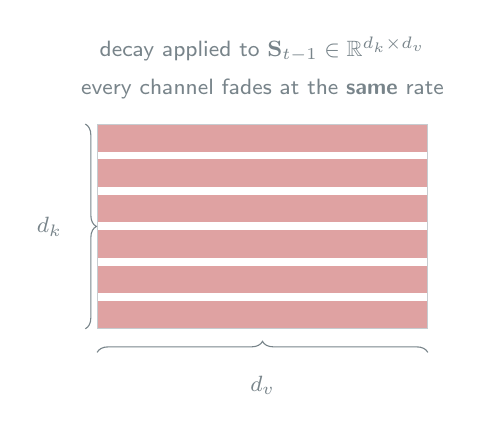
\begin{tikzpicture}[font=\footnotesize]
  \node[dim,align=center] at (2.1,3.55) {decay applied to $\St_{t-1}\in\R^{d_k\times d_v}$};
  \node[dim,align=center] at (2.1,3.05) {every channel fades at the \textbf{same} rate};
  \foreach \i in {0,...,5}
    \fill[gatered,opacity=0.42] (0,{0.45*\i}) rectangle (4.2,{0.45*\i+0.35});
  \draw[mat,fill=none] (0,0) rectangle (4.2,2.6);
  \draw[decorate,decoration={brace,amplitude=4pt},draw=mute]
    (-0.15,2.6) -- (-0.15,0) node[midway,left=5pt,dim] {$d_k$};
  \draw[decorate,decoration={brace,amplitude=4pt},draw=mute]
    (0,-0.3) -- (4.2,-0.3) node[midway,below=5pt,dim] {$d_v$};
\end{tikzpicture}}
\vspace{0.25cm}
{\footnotesize\color{mute}\centering A single gate cannot keep one channel while flushing another.\par}
\end{column}
\end{columns}
\end{frame}

% ======================================================================
\begin{frame}[t]{Kimi Delta Attention (KDA): fine-grained gating}
\vspace{0.1cm}
{\small Promote the scalar \g{$\alpha_t$} to a \hi{per-channel vector} $\g{\bm{\alpha}_t}\in[0,1]^{d_k}$.}

\begin{columns}[T]
\begin{column}{0.54\textwidth}
\vspace{0.15cm}
{\small
\[
  \St_t=\big(\mathbf{I}-\beta_t\bm{k}_t\bm{k}^\top_t\big)\g{\Diag(\bm{\alpha}_t)}\St_{t-1}+\beta_t\bm{k}_t\bm{v}^\top_t
\]
\vspace{-0.45cm}
\[
  \bm{o}_t=\St^\top_t\bm{q}_t\in\R^{d_v}
\]}
\vspace{-0.1cm}
\fig[2.2cm]{%
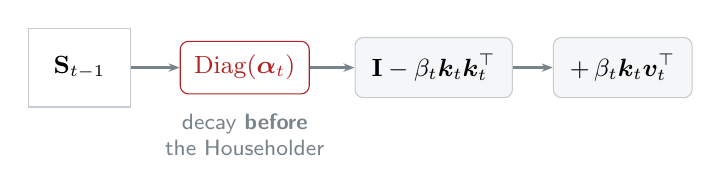
\begin{tikzpicture}[font=\small]
  \node[mat,minimum width=1.3cm,minimum height=1.0cm] (s0) at (0,0) {$\St_{t-1}$};
  \node[gate] (a) at (2.1,0) {\g{$\Diag(\bm{\alpha}_t)$}};
  \node[blk] (h) at (4.5,0) {$\mathbf{I}-\beta_t\bm{k}_t\bm{k}^\top_t$};
  \node[blk] (w) at (6.9,0) {$+\,\beta_t\bm{k}_t\bm{v}^\top_t$};
  \foreach \a/\b in {s0/a,a/h,h/w} \draw[arr] (\a) -- (\b);
  \node[dim,align=center] at (2.1,-0.85) {decay \textbf{before}\\ the Householder};
\end{tikzpicture}}
\vspace{0.25cm}
{\small\textbf{Parameterization} (low-rank, like the output gate):
\[
  \g{\bm{\alpha}^h_t}=f\big(\mathbf{W}^{\uparrow}_{\alpha}\mathbf{W}^{\downarrow}_{\alpha}\bm{x}_t\big)\in[0,1]^{d_k},
  \quad \beta^h_t=\sigma(\mathbf{W}^h_\beta\bm{x}_t)
\]}
\end{column}

\begin{column}{0.46\textwidth}
\vspace{0.3cm}
\fig[3.0cm]{%
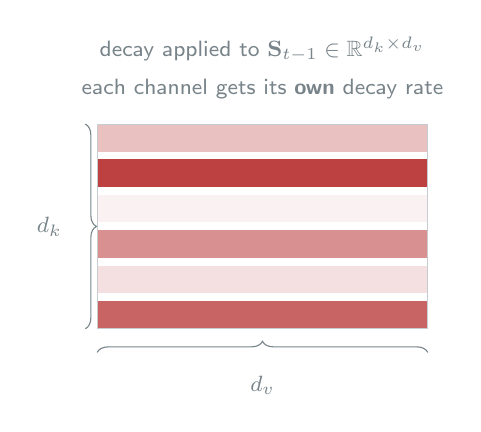
\begin{tikzpicture}[font=\footnotesize]
  \node[dim,align=center] at (2.1,3.55) {decay applied to $\St_{t-1}\in\R^{d_k\times d_v}$};
  \node[dim,align=center] at (2.1,3.05) {each channel gets its \textbf{own} decay rate};
  \foreach \i/\o in {0/0.70,1/0.14,2/0.50,3/0.06,4/0.86,5/0.28}
    \fill[gatered,opacity=\o] (0,{0.45*\i}) rectangle (4.2,{0.45*\i+0.35});
  \draw[mat,fill=none] (0,0) rectangle (4.2,2.6);
  \draw[decorate,decoration={brace,amplitude=4pt},draw=mute]
    (-0.15,2.6) -- (-0.15,0) node[midway,left=5pt,dim] {$d_k$};
  \draw[decorate,decoration={brace,amplitude=4pt},draw=mute]
    (0,-0.3) -- (4.2,-0.3) node[midway,below=5pt,dim] {$d_v$};
\end{tikzpicture}}
\vspace{0.2cm}
{\footnotesize
\begin{itemize}
  \item Per-channel forgetting \emph{and} positional awareness.
  \item DPLR expressiveness, but tying $\bm{a}_t,\bm{b}_t$ to $\bm{k}_t$ makes the kernel $\sim$2$\times$ faster.
\end{itemize}}
\end{column}
\end{columns}
\end{frame}

% ======================================================================
\begin{frame}[t]{Summary of state updates}
\vspace{0.7cm}
\begin{center}
{\small
\begin{tabular}{@{}llll@{}}
\toprule
\textbf{Model} & \textbf{State update} & \textbf{Decay} & \textbf{Memory}\\
\midrule
Linear attn.
  & $\St_{t-1}+\bm{k}_t\bm{v}^\top_t$
  & none
  & $d_k\!\times\!d_v$\\[0.35em]
DeltaNet
  & $(\mathbf{I}-\beta_t\bm{k}_t\bm{k}^\top_t)\St_{t-1}+\beta_t\bm{k}_t\bm{v}^\top_t$
  & none
  & $d_k\!\times\!d_v$\\[0.35em]
Gated DeltaNet
  & $\g{\alpha_t}(\mathbf{I}-\beta_t\bm{k}_t\bm{k}^\top_t)\St_{t-1}+\beta_t\bm{k}_t\bm{v}^\top_t$
  & scalar \g{$\alpha_t\in[0,1]$}
  & $d_k\!\times\!d_v$\\[0.35em]
\textbf{KDA}
  & $(\mathbf{I}-\beta_t\bm{k}_t\bm{k}^\top_t)\g{\Diag(\bm{\alpha}_t)}\St_{t-1}+\beta_t\bm{k}_t\bm{v}^\top_t$
  & \g{$\bm{\alpha}_t\in[0,1]^{d_k}$} per channel
  & $d_k\!\times\!d_v$\\
\bottomrule
\end{tabular}}
\end{center}

\vfill
\takeaway{State size is $O(1)$ in every row; the variants differ only in the transition matrix.}
\vspace{0.4cm}
\end{frame}

\sectionslide{Section 3}{Making the MLP Cheaper}

\end{document}
